% GENERATED COPY -- do not edit.
% Source: report-common/gantt.tex; run `python report-common/sync.py`.
% Shared by every report: the semester plan. See report-common/diagrams.tex
% for how these shared fragments are kept in step.
%
% Deliberately only the landscape figure, with the explanation in the caption:
% any body text here is orphaned on a near-empty portrait page, because
% \begin{landscape} forces a page break.

\begin{landscape}
\begin{figure}[H]
    \centering
    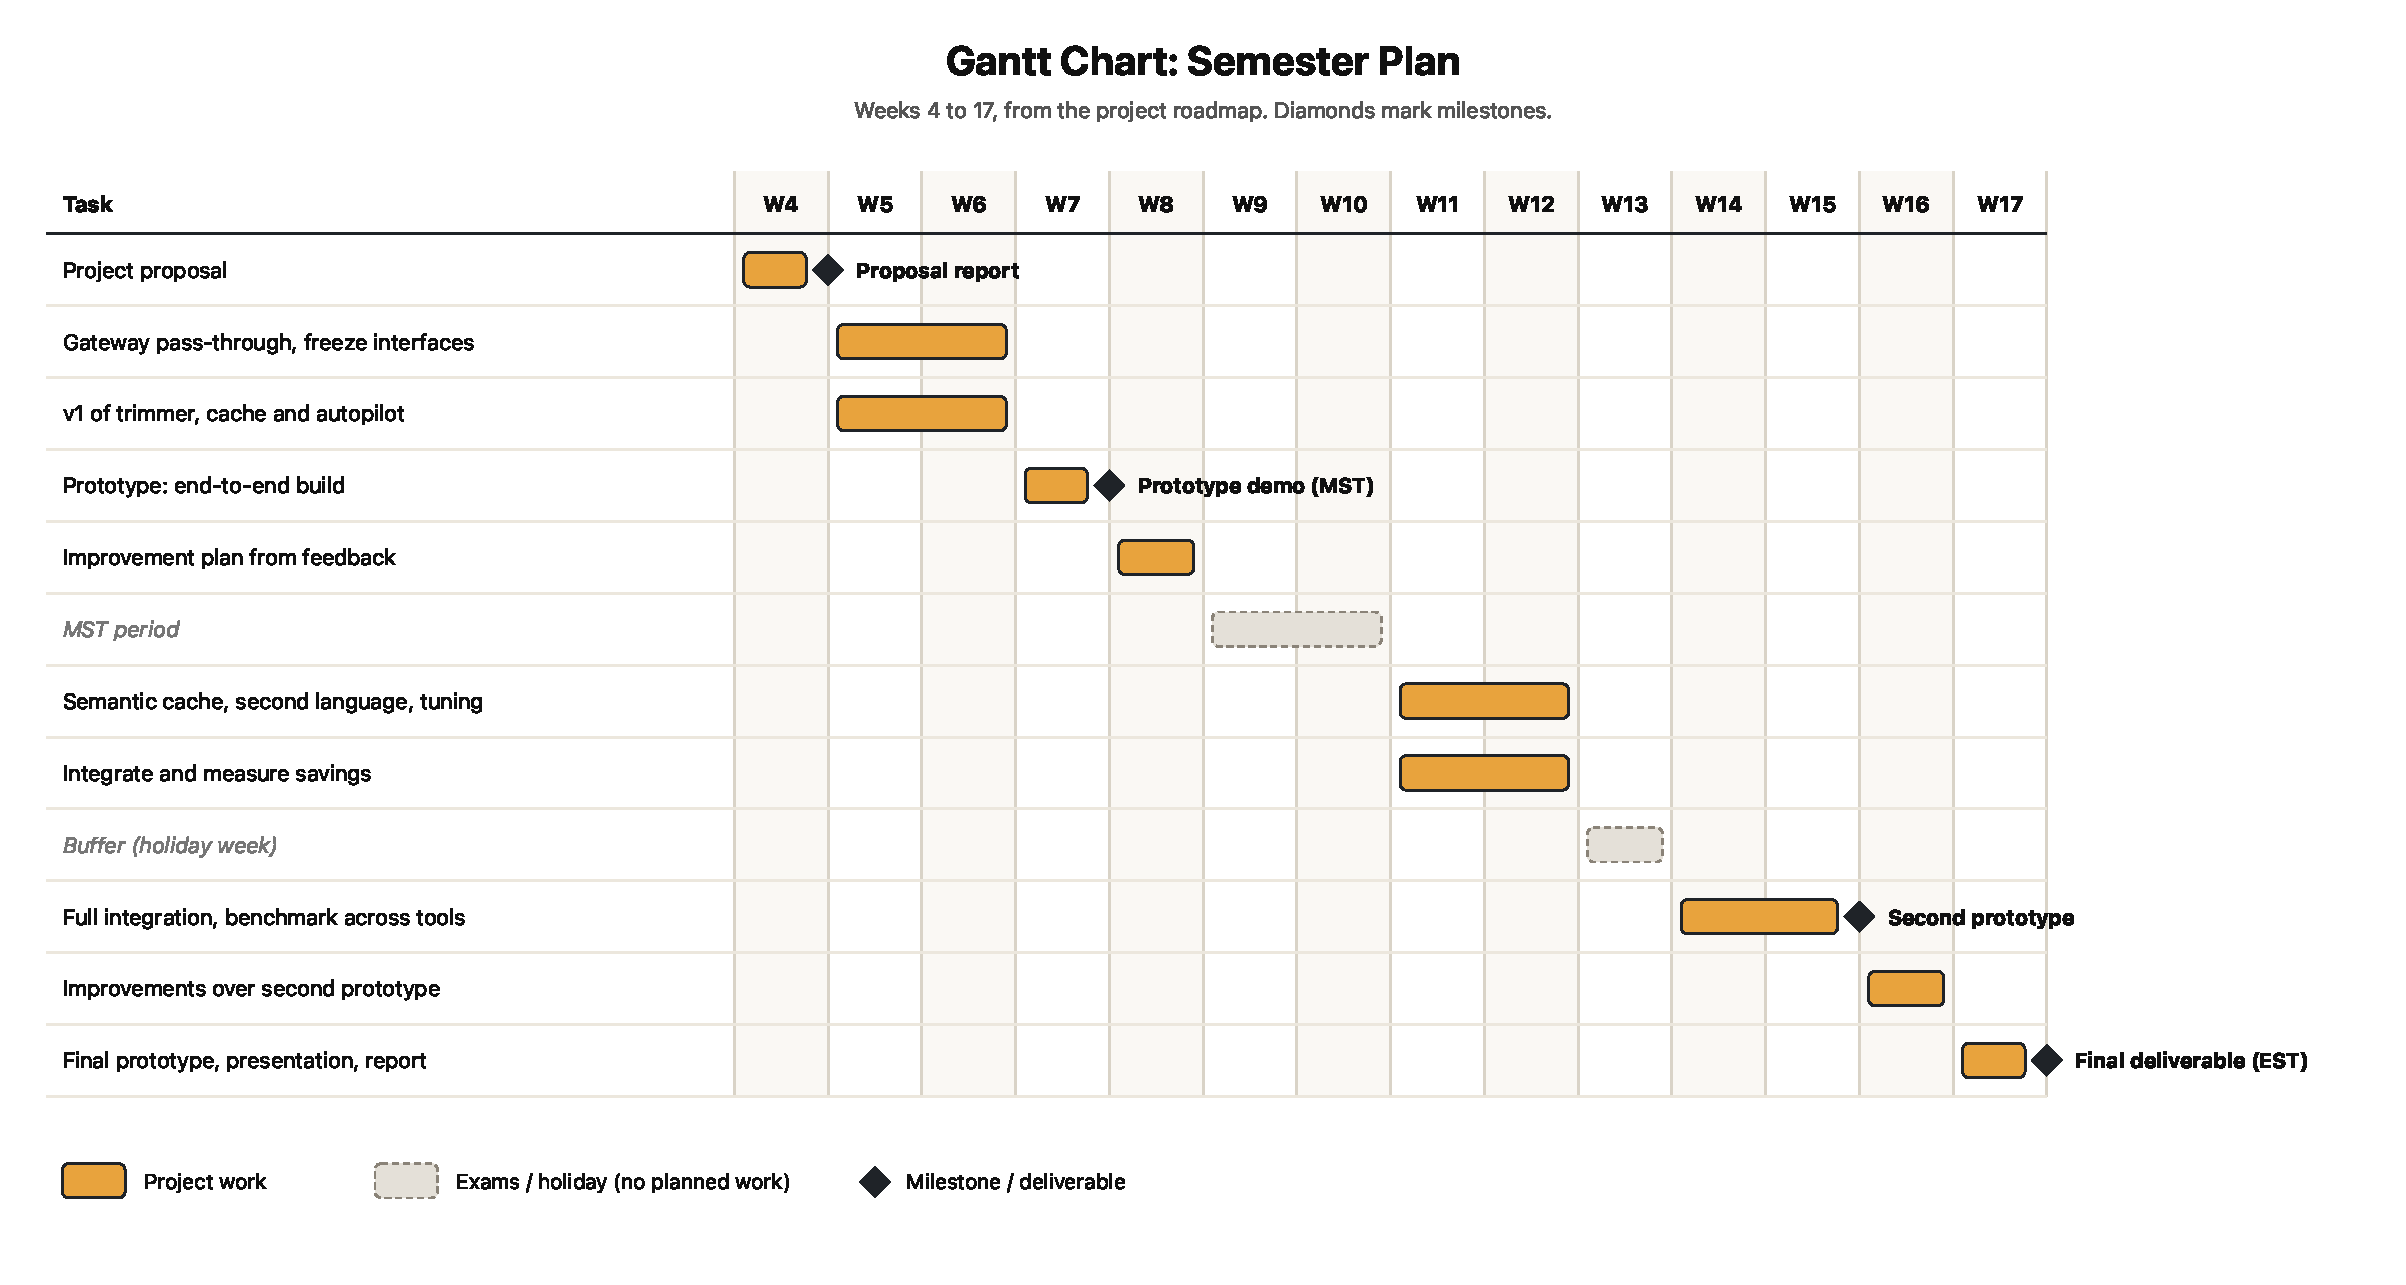
\includegraphics[width=\linewidth, height=0.80\textheight, keepaspectratio]{gantt-chart}
    \caption[Semester plan for weeks 4 to 17.]{Semester plan for weeks 4 to 17.
             Diamonds mark the four scheduled deliverables: the proposal (W4),
             the prototype demo at the mid-semester test (W7), the second
             prototype (W14 to W15) and the final deliverable at the
             end-semester test (W17). Shaded weeks carry no planned work: the
             MST period (W9 to W10) and the holiday buffer (W13). The same
             schedule is kept as a table on the project site under Roadmap.}
    \label{fig:gantt}
\end{figure}
\end{landscape}
